% !Mode:: "TeX:UTF-8"

% !TEX root = ../main.tex

\chapter{基于属性的凭证在车辆自组网中的应用}[Application in VANETs]

在前面的章节中,我们主要介绍了基于属性的凭证的相关概念,以及在保护个人隐私方面所发挥的作用。
现实生活中有很多需要身份验证的场景,大多数的场景都缺少一种保护用户隐私的措施,这会给用户本身带来很大的安全隐患。
如何在确保通过验证的同时又不泄露个人的隐私信息,这已成为隐私保护领域关注的热点问题之一。
车辆自组网环境就属于这类场景。

\section{车辆自组网}[Enviroment]

车辆自组网作为智能交通系统的重要组成单元,主要是为了解决道路安全问题以及为驾乘人员提供便利而出现的。
与现在热门的无人驾驶有很大不同,车辆自组网更侧重于提供辅助驾驶,主要集中在对车辆间通信的研究。
这个概念很大程度上来源于物联网,因此车辆自组网可以看做是实现车联网的一个必要组件。

车与车之间通过频繁的信息交换,可以用来实现智能化的交通系统。
想象在车辆自组网的环境中,我们可以通过接收其他车辆发送过来的信息,判断前面道路的拥挤状况,然后就可以挑选出最优的驾驶路线。
在一些比较复杂的路况下,我们还可以通过获取附近车辆的速度与它们的位置等信息,在判断可能出现危险的情况下,及时发出警告或者车辆主动采取紧急制动措施,这样就能避免许多交通事故的发生。
从这种角度来看,车辆自组网与无人驾驶是相辅相成的关系,如果能很好地实现车辆自组网,那么也将会推动无人驾驶的发展。

在车辆自组网的环境中,每辆车都要求配备一个称为车载通信单元(On-Board Unit,OBU)的设备。
这些设备可以将车辆的速度,位置及当前的路况等信息进行广播。
道路两旁会设置一些路边单元(Road-Side Units,RSUs),这些路边单元与交通管理中心(Transportation Regulation Center,TRC)相互联通,它们也可以与车辆进行通信,以提供交通服务等信息。

因此,我们可以把车辆自组网中的通信方式粗略分为两类,一类是车辆与车辆之间的通信,即V2V(Vehicle to Vehicle);另一类是车辆与RSUs这类的基础设施之间的通信,即V2I(Vehicle to Infrastructure)。
整个车辆自组网中的环境如图4-1所示。
目前的车辆自组网通信还没有形成统一的标准,比较有影响力的有基于DSRC(Dedicated Short Range Communications)技术的IEEE802.11p标准和基于LTE蜂窝网络的LTE-V标准。
以IEEE802.11p标准为例,它是在IEEE802.11的基础上专门针对车用通信网络改良的。
IEEE802.11p标准利用DSRC技术完成V2V和V2I两种通信方式。
DSRC是一种国际上通用的专门适用于车辆通信的技术,最早是由美国材料与实验协会于1992年提出,现在被广泛应用于电子不停车收费系统(Electronic Toll Collection,ETC)中。DSRC拥有延迟低、兼容性强等特点,已获得大多数车辆企业的支持。
DSRC技术要求车辆以一定的时间间隔(100到300毫秒)周期性地广播与交通相关的信息\cite{zhang2008raise}。
因此如何保证这些信息是可被验证的,这已经成为车辆自组网中需要关注的首要问题。

\begin{figure}[h]
\centering
\includegraphics[width = 0.9\textwidth]{V2X_v3_1}
\caption{车辆自组网的环境}
\end{figure}

正因为车辆自组网处于一种公开的环境中,所以很容易受到恶意的攻击。
如果恶意的车辆广播一些虚假的交通事故或交通堵塞信息,将会给其他车辆造成误导,从而破坏交通系统的秩序。
为了保障整个交通系统的安全,最简单的方法就是强制在广播的信息中附加可验证的车辆信息(如数字签名)。
这种做法提高了传播恶意信息的代价,虽然能确保整个交通系统的安全,但同时也在一定程度上泄漏了车辆的隐私。
% 给个引文 或者举个例子
现在的车联网通信标准首要考虑的是如何确保道路的安全,比如DSRC技术提供了ECDSA数字签名算法来保证信息的可验证性\cite{zhang2008raise}。
一些工作\cite{da2012examining,zhang2008raise}指出这种仅使用数字签名的方式会给车辆的隐私带来一定的风险。

隐私和安全是车辆自组网中重点关注的议题,隐私注重的是车辆的身份等信息不能完全暴露,而安全通常指的是交通系统的安全,它意味着车辆广播的信息是要能被认证。
欲保护用户的隐私,那么车辆在与其它车辆或RSUs进行通信的时候,需要保持一种匿名的状态。
但如果是完全匿名的话,一些恶意的车辆就会肆无忌惮地广播虚假的信息,这样会给整个交通系统带来不好的影响。
另外,在出现一些意外情况(如交通事故)时,我们还需要能够还原出信息签名者的真实身份。
因此在车辆自组网中,在满足可验证性的前提下,还需要满足匿名性及可追踪性。
从这些角度来看,我们会发现车辆自组网的环境与基于属性的凭证系统有许多相似的地方。

\begin{table}[htbp]
\bicaption[table1]{}{基于属性的凭证系统与车辆自组网环境的比较}
\vspace{0.5em}\centering\wuhao
\begin{tabular}{ccccc}
\toprule[1.5pt]
 & 基于属性的凭证系统 & 车辆自组网环境 \\
\midrule[1pt]
 需要认证的内容 & 用户的属性信息 & 车辆的速度,路况等信息 \\
 需满足的基本性质 & 可验证性,匿名性 & 可验证性,匿名性,可追踪性,实时性 \\
 可以信任的实体 & 凭证发行机构 & 交通管理中心 \\ 
\bottomrule[1.5pt]
\end{tabular}
\end{table}

通过表4-1,我们可以发现车辆自组网的环境与基于属性的凭证系统有着很多相似的地方。
除此之外,实时性是车辆自组网环境中必须要满足的一个性质,尤其是当车辆密度比较大或车辆处于高速移动的状态,实时性就显得尤其重要。
如果直接把现有的基于属性的凭证系统移植到车辆自组网系统中,则会因为无法保证实时性的要求而不可行。
如何设计出一个针对车辆自组网场景的方案,既能确保交通系统的安全和车辆的隐私,又能满足在特定场景中能还原用户的真实身份的需求,还能确保整个过程的高效性,是现在面临的主要问题。

\section{相关工作}[Related Schemes]

在车辆自组网研究的早期阶段,大多数的研究工作是围绕着如何确保信息的可验证性。
因此很自然地就有了使用数字签名的方法来防止信息的伪造\cite{el2002security}。
但这种方案显然会暴露隐私,因为用来验证信息的公钥可以对应看做车辆的身份信息\cite{petit2015pseudonym,da2012examining}。
近些年的研究工作开始集中在隐私保护方面,这些工作大多是基于假名的方式。

根据假名表示的方法不同,这些方案大致分为四类\cite{petit2015pseudonym}:
第一类是基于传统的公钥密码学,第二类是使用基于身份的密码学。
严格来说这两种方案都是公钥密码体制,核心思想都是用户自己申请多个公钥,然后通过频繁更换公钥的方式来维持匿名的状态。
在这里,假名可以看做是由公钥来表示的。
每个公钥会限制使用日期或使用次数,从而切断了公钥与真实身份之间的关联性。
前者是基于公钥基础设施(Public Key Infrastructure,PKI),因此需要使用公钥证书对车辆的公钥进行管理。
后者采用基于身份的密码学,由于不需要使用公钥证书,从而简化了公钥签发的过程。

然而,这种依赖频繁地更换假名保证匿名的方法并不能完全地阻止对身份的追踪\cite{wiedersheim2010privacy}。
因此许多工作开始关注如何更换假名,出现了像Mix-Context-Based、Mix-Zone-Based\cite{jemaa2017study,ying2013dynamic,lu2012pseudonym}等更换假名的策略。
但是这些策略都存在一定的局限性,并不能从根本上解决问题。

第三类方案是基于群签名的,这种方案的好处是不用考虑假名更换的问题。
群签名中存在着一个群管理员,群管理员可以添加或移除群成员,然后群成员可以使用自己的私钥对信息生成一个群签名。
群成员在验证签名的时候使用的是群公钥,因此能很好地满足匿名的特性,符合车辆自组网中对可验证性及匿名性的要求。
但群签名最大的弊端在于群管理员的权力过大,群管理员可以根据签名信息直接获取签名者的身份。
因此,有些方案提出使用RSUs作为群管理员\cite{hao2011distributed,park2011rsu},但由于RSUs长期处于公共环境中,很容易遭到攻击与破坏。
将RSUs作为群管理员,在实际中会给车辆的身份信息带来一定的风险。

第四类方案是基于对称密码学,这类方案是使用消息验证码来保障信息的完整性\cite{petit2015pseudonym,choi2005balancing}。
与公钥密码学最大的不同之处在于,对称密码学中签名与认证使用的密钥是相同的。
虽然此类方案的计算效率比较高,但由于使用的密钥是相同的,因此很难实现可追踪性。
大部分的方案都要求使用RSUs完成信息的验证与转发,系统的安全会严重依赖于RSUs。
而且由于RSUs的计算及存储能力有限,可能会成为整个车辆自组网的性能瓶颈。

与群签名类似的还有基于环签名的方案\cite{xiong2010efficient,chaurasia2011conditional,zeng2015privacy},相比基于群签名的方案,环签名中因为没有群管理员的存在,相对来说更加安全。
在这些方案中,车辆可以自由地生成签名,而不用依赖群管理员。
由于环签名本身是一种完全匿名的签名方案,为了满足车辆的可追踪性,需要在环签名的方案上进行一些改进,将这种完全匿名变为有条件的匿名\cite{张建明2012车辆自组网的位置隐私保护技术研究}。
正因为没有了群管理员的控制,车辆可以自发产生一个基于某个环上的签名。
但同时由于这种不可控制性,车辆自发生成的签名很可能是无效的。
现有的基于环签名的方案都没有讨论如何确保环成员的有效性,因为缺少适当的验证操作,车辆很容易会产生一个无效的签名,这会给整个交通系统带来不确定因素。

\section{构造方案}[Proposal Scheme]

通过前面的介绍,我们知道在车辆自组网中,车辆发送的消息一方面要能够被验证,另一方面要保证不泄漏隐私信息。
看上去与基于属性的凭证中对属性的要求很类似。但二者之间也存在着很明显的差别。

在基于属性的凭证系统中,消息的有效性是靠凭证发行机构的签名保证的;
而车辆自组网的环境中,车辆不能频繁地与TRC通信,因此信息的签名过程是由车辆自己完成的。
那么,我们可不可以直接使用一种具有匿名性质的签名体制来同时保证匿名性和可验证性呢?

考虑到车辆自组网的特殊结构,环签名看上去是很不错的解决方案。
但是环签名具备极高的自发性,如果车辆可以自由收集其他车辆的公钥并对消息进行签名的话,很容易由于环中存在失效的成员而使签名无效。
现有的基于环签名的方案\cite{xiong2010efficient,chaurasia2011conditional,zeng2015privacy}都没有考虑这个问题。
在这些方案中,为了突出环签名的优势,直接移除了RSUs,没有考虑V2I能发挥的作用。
那么我们为什么不能将RSUs放到基于环签名的方案中呢?
如果可以将RSUs融入进去,并使用V2I的方式分配环成员,是不是就可以解决这个问题呢?

因此我们希望将RSUs与基于环签名的方案结合。
在车辆进入某一区域时,需要通过向区域内的RSUs发出请求来获取一个成员列表。
RSUs在验证车辆的身份后,向其分配一个有效的成员列表。
车辆收到这个列表后,便可以使用环签名的方式对需要发送的信息进行签名。

虽然环签名可以同时满足可验证性和匿名性这两个基本性质,但环签名带来的匿名是无条件的。
因此我们需要在签名上面附加一些可追踪的信息。
以往的许多方案中,追踪这一功能是由TRC完成的,即TRC拥有权力可以直接根据生成的签名等信息还原出签名者的真实身份。
但在实际中并不完全是这样,想象在出现交通事故时,一般是需要有执法部门完成对信息源的追踪,TRC应该是起到辅助追踪的作用。
因此我们引入了执法机关(Law Enforcement)这样一个实体,利用这种机构完成签名的追踪,并解析出签名者的假名。
如果有进一步的需要,执法机关还可以根据这个假名从TRC的数据库中还原出其对应的真实ID,并进行撤销操作。

要合理使用密码学的工具来构建这样一个方案不是容易的事情,一方面我们需要避开以前方案的劣势,另一方面我们需要在效率上满足一定的要求。这就需要与其它方案进行对比,还要找到合适的衡量方法体现方案高效率的特点。另外,在说明我们方案满足的性质的时候,需要对满足的这些性质进行合理的论证,有必要的话还可以采取形式化的证明方式。
为了方便证明,我们也可以引入随机预言机模型。
在证明之前,通常需要引入合理的假设前提,并给出攻击者的攻击模型。

按照这样的思路,首先我们把车辆的假名按照从生成到撤销划分为六个阶段,每个阶段包括一些具体的操作过程,如图4-2所示。

\begin{figure}[h]
\centering
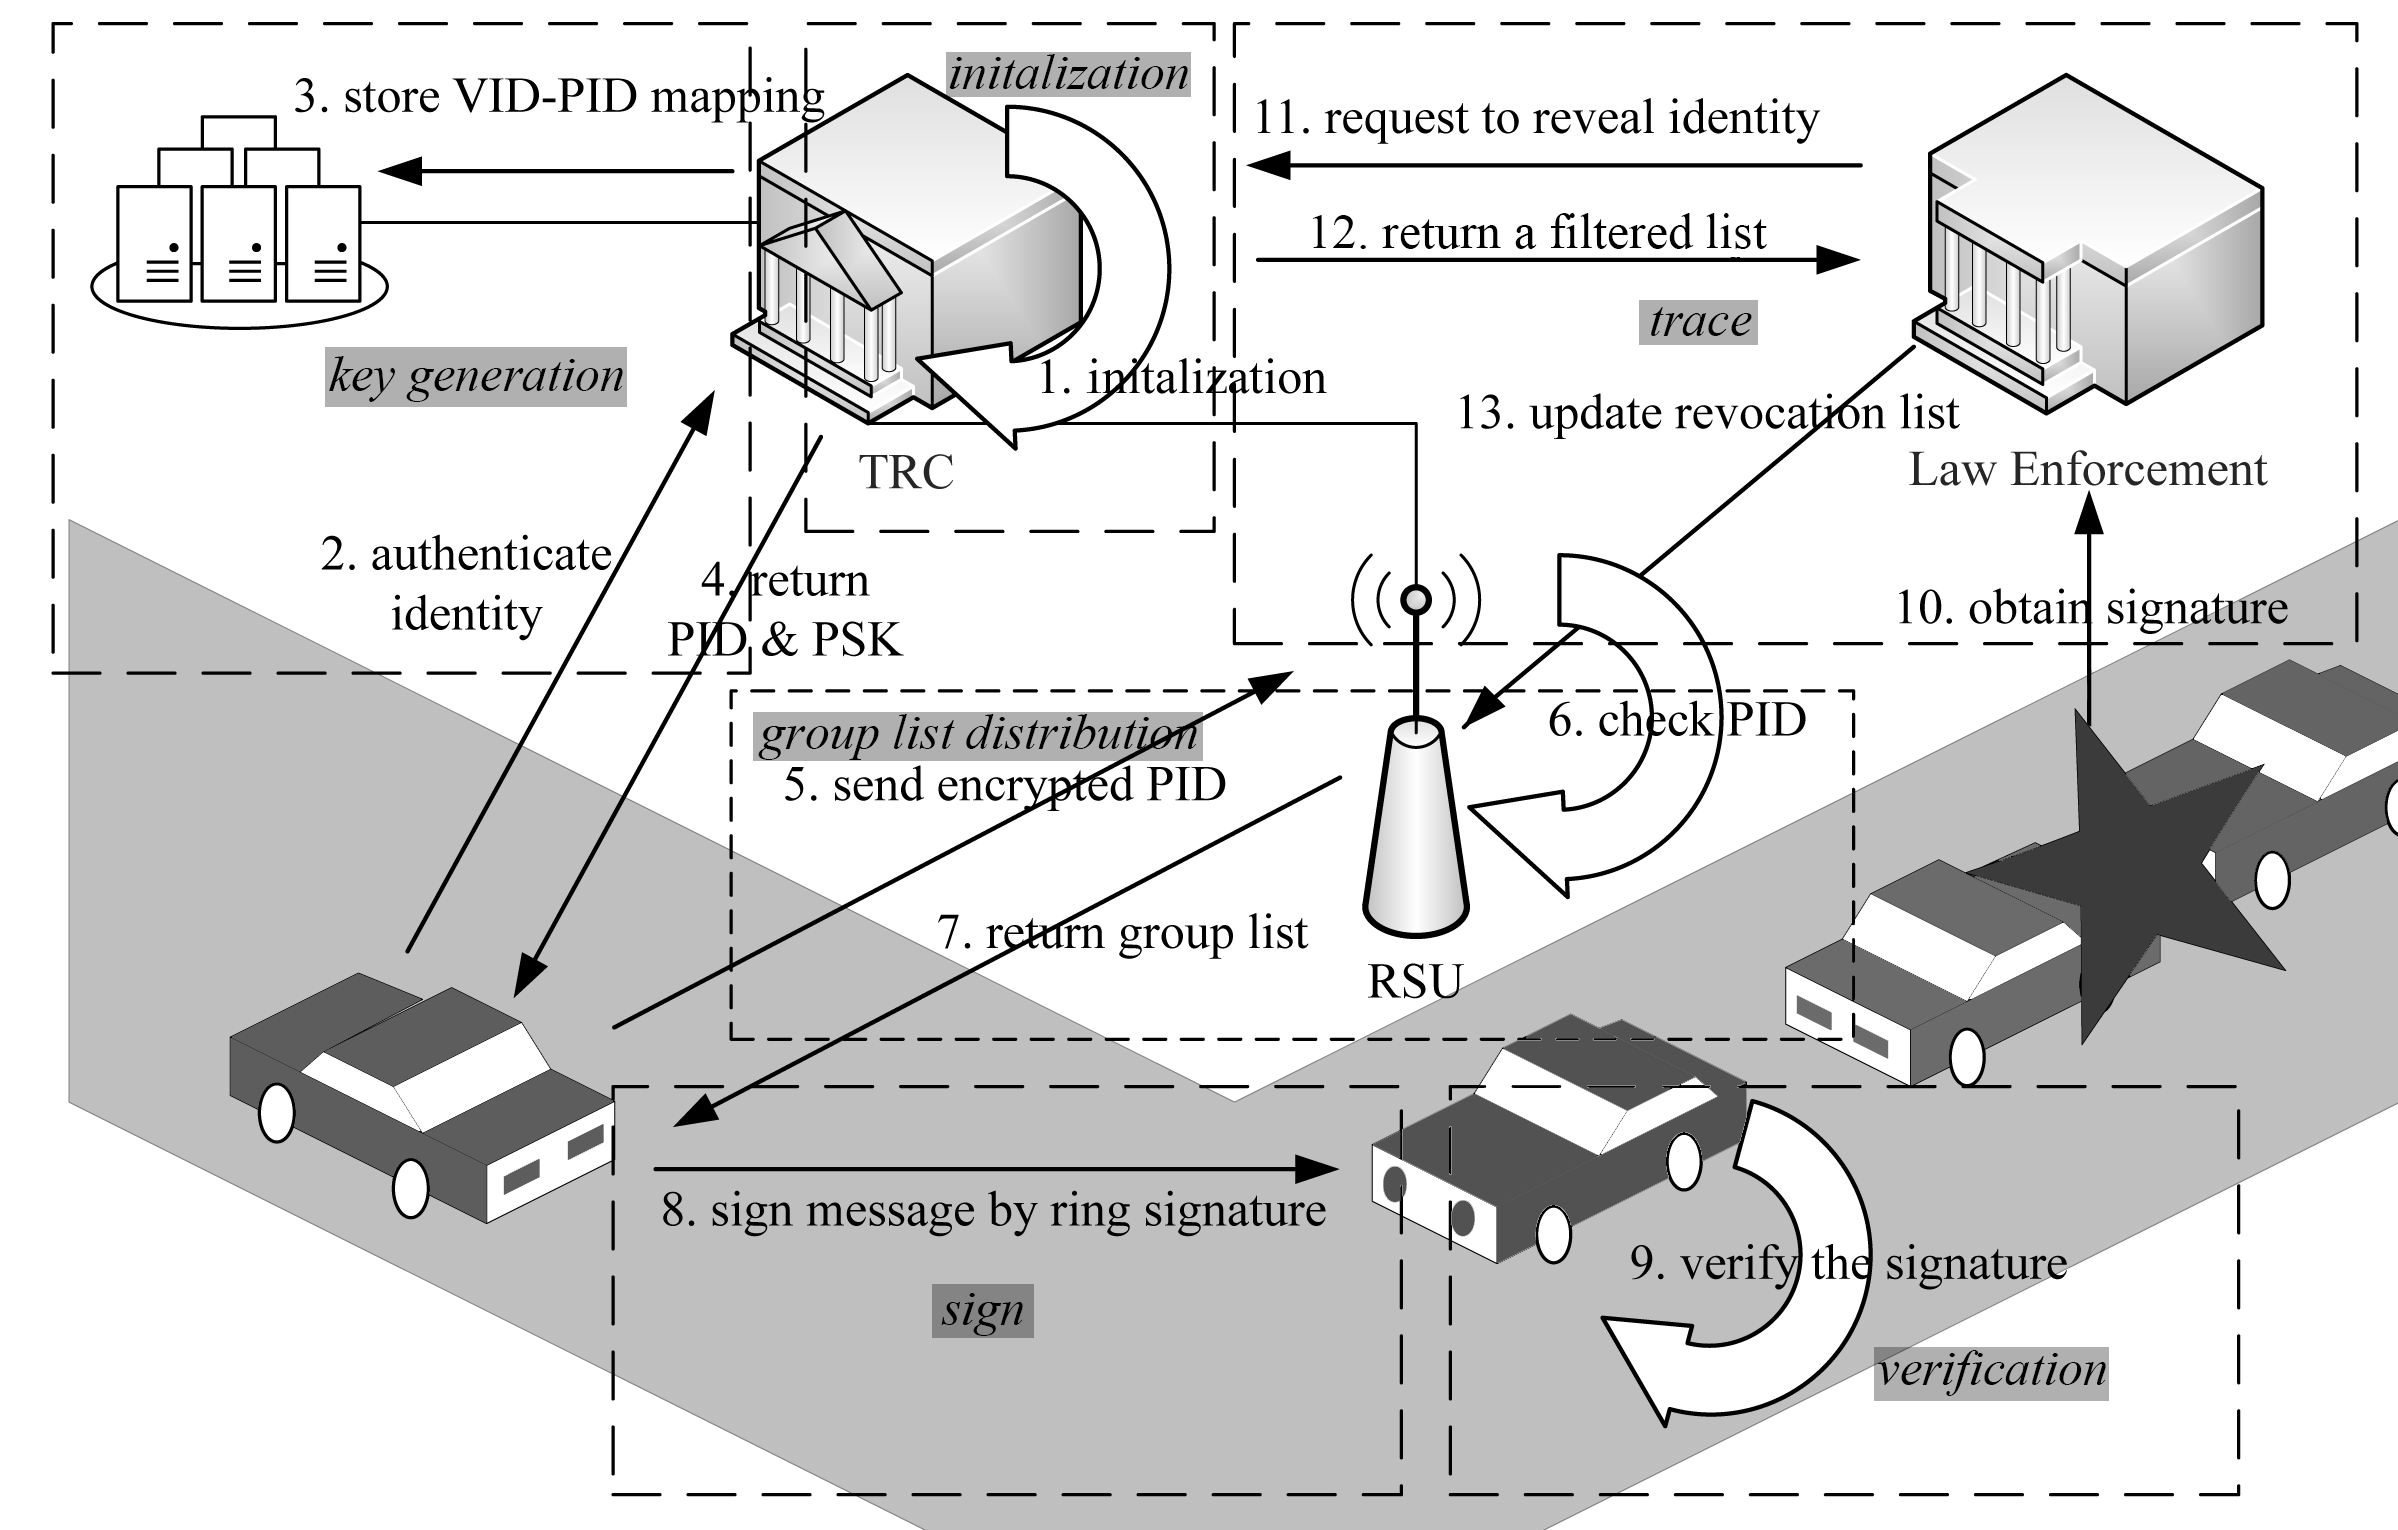
\includegraphics[width = 0.9\textwidth]{V2X_v6}
\caption{方案构造}
\end{figure}

从图中可以看到,在我们的方案中共有4类参与者,它们分别是交通管理中心(TRC),执法机关,配备了OBUs的车辆以及道路两旁的RSUs。
在充分考虑到RSUs特殊身份的情况下,我们提出使用基于身份的加密方案来完成车辆向RSUs的请求列表过程,利用对称密码机制完成RSUs的成员列表分配过程。

根据双线性映射的性质,保证在一次交互之后,双方可以获得相同的密钥信息。
为了完成追踪,我们在为签名的内容附加一个可追踪的$tag$。
为了方便说明,我们把需要使用的符号以及它所表示的含义列举出来,如表4-2所示。

\begin{table}[htbp]
\bicaption[table2]{}{符号及其含义}
\vspace{0.5em}\centering\wuhao
\begin{tabular}{ccccc}
\toprule[1.5pt]
 符号 & 含义 \\
\midrule[1pt]
 $s$ & TRC的主私钥 \\
 $PK$ & TRC的公钥\\
 $s_{trac}$ & 执法机关的私钥\\
 $PK_{trac}$ & 执法机关的公钥\\
 $PP$ & 公共参数\\
 $VID$ & OBUs的真实ID\\ 
 $PID$ & OBUs的公钥(也称作假名)\\
 $PSK$ & OBUs的私钥\\
 $RID$ & RSUs的公钥\\
 $RSK$ & RSUs的私钥\\
 $k_{i-j}$ & i 与 j 之间的共享公钥\\
 $L$ & 成员列表,用于环签名\\
 $t_d$ & $L$的失效时间\\
 $t$ & 签名的时间戳\\
 $tag$ & 用于追踪的标签\\
 $a||b$ & 将字符串$a$与$b$进行连接\\
\bottomrule[1.5pt]
\end{tabular}
\end{table}

每一个步骤的操作细节我们将按照初始化,密钥生成,成员列表分配,签名,验证和追踪这六个阶段分别进行介绍。

\subsection{初始化}[Setup]

系统的初始化过程包含一个$\mathsf{Setup}$算法,这个算法是由TRC执行的。
由于我们的方案是利用双线性映射来实现的,初始化的结果就是生成了一个双线性映射及相关的一些参数。
\begin{itemize}
  \item $(pp,s)\leftarrow\mathsf{Setup}(1^\kappa)$:在初始阶段,对于给定的安全参数$\kappa$,算法$\mathsf{Setup}(\cdot)$可以生成公共参数$pp$和TRC的私钥$s$。其中$s\in_R\mathbb{Z}^*_q$是随机选取的,$pp=(\mathbb{G}_1,\mathbb{G}_T,P,q,e,PK,H_1,H_2)$。
  $\mathbb{G}_1$与$\mathbb{G}_T$均为阶数为$q$的循环群,$e:\mathbb{G}_1\times\mathbb{G}_1\rightarrow\mathbb{G}_T$是一个双线性映射。
$P$是$\mathbb{G}_1$的一个生成元,$PK$又被称为TRC的公钥,且有$PK=s\cdot P$。
$H_1$和$H_2$是两个密码哈希函数,且$H_1:\{0,1\}^*\rightarrow\mathbb{G}_1$,$H_2:\{0,1\}^*\rightarrow\mathbb{Z}_q^*$。
\end{itemize}

在完成初始化过程之后,TRC可以将$pp$进行公开,并保管好私钥$s$。
为了实现可追踪性,执法机关需要根据初始化后的公开参数$pp$生成对应的密钥对$(s_{trac},PK_{trac})$。
其中$s_{trac}\in_R\mathbb{Z}_q^*$,为执法机关的私钥,在进行追踪时会用到;$PK_{trac}=s_{trac}\cdot P$,作为执法机关的公钥,可以事先载入到车辆的OBUs设备中。

\subsection{密钥生成}[Keygen]

在初始化完成之后,RSUs和配备有OBUs的车辆就可以从TRC处获取自己的密钥对。
在这里我们需要做一个假设,即每辆车的OBU中都存在一个硬件安全模块(Hardware Security Module,HSM)\cite{tzeng2017enhancing}。
存储在HSM中的信息不会遭到篡改,同时一些与密码学有关的操作如加密,签名等也是在HSM中完成。

系统中,每一辆车都有一个唯一的身份编号,我们用$VID$来表示。
对于真实身份为$VID_\ell$的车辆,它可以通过向TRC提交$VID_\ell$来获取自己的密钥对。
TRC在收到$VID_\ell$之后,开始执行$\mathsf{KeyGen}(VID_\ell)$算法,并把生成的密钥对及$pp$载入到HSM中。

\begin{itemize}
  \item $(PID_\ell,PSK_\ell)\leftarrow\mathsf{KeyGen}(VID_\ell)$:输出的$PID_\ell$和$PSK_\ell$分别代表着$VID_\ell$的公钥和私钥。
  其中$PID_\ell=H_1(VID_\ell||salt)$,$PSK_\ell=s\cdot PID_\ell$。$salt$是随机选取的,即$salt\in_R\mathbb{Z}_q^*$。
  为了实现可追踪性,执法机关的公钥$PK_{trac}$需要事先存储在HSM中。
  TRC还会把$PID_\ell$与$VID_\ell$对应起来保存在数据库中。
\end{itemize}

类似地,对于真实身份为$ID_j$的RSU来说,它获取到的密钥对为$(RID_j,RSK_j)$,其中$RID_j=H_1(ID_j)$,$RSK_j=s\cdot RID_j$。
与车辆编号$VID_\ell$不同,RSU的身份编号$ID_j$是可以直接公开的。
因此对于车辆而言,某一区域内的RSUs信息均为可查的。

这里RSUs与OBUs获取假名的方式略有不同,OBUs获取到的假名是在$VID$的基础上加盐哈希产生的,目的是车辆可以在不用更换$VID$的情况下可以从TRC处获取新的假名,满足车辆定期更换假名的需求。

由于RSUs是公共设施,而且IDs都是可以公开查询的,直接使用哈希获取假名的方式能够容易让其它车辆进行检验。
即当车辆进入某一区域时,由于事先知道这一区域RSUs的IDs,便可直接使用哈希函数$H_1$来计算RSUs的公钥(假名)。
这样就可以使用此公钥进行数据的加密,从而避免出现与伪装成RSUs的设备进行通信的情况。

\subsection{成员列表分配}[groupList]

当车辆进入一个区域时,它首先需要向该区域内的RSUs发送请求,在请求通过后,RSUs再向其发送一个成员列表。
为了方便说明,不妨假设车辆$VID_\ell$在与$RSU_j$进行通信,在这一过程中,我们使用第二章2.4节中的基于身份的加密方案,并使用$\mathsf{Enc}$和$\mathsf{Dec}$分别表示此方案的加密和解密算法\cite{boneh2001identity}。
另外,我们使用$\mathcal{ENC}(\cdot)$,$\mathcal{DEC}(\cdot)$,$\mathcal{HMAC}(\cdot)$分别表示对称密码体制下的加密算法、解密算法以及消息验证码算法。
具体的通信过程可以分为以下几个步骤:

\begin{itemize}
  \item $RSU_j$ 在该区域内广播自己的公钥$PID_j$;
  \item $VID_\ell$进入该区域后,首先可以获得$PID_j$。
  由于$ID_j$是公开的,因此$VID_\ell$可以直接用哈希算法判断$PID_j$的真实性。
  之后$VID_\ell$就可以使用$PID_j$加密自己的假名,即$C=\mathsf{Enc}(PID_\ell,RID_j)$,并把加密后的密文$C$发送给$RSU_j$;
  \item $RSU_j$在收到密文$C$之后后,可以利用自己的私钥计算出$VID_\ell$的公钥,即$PID_\ell=\mathsf{Dec}(C,RSK_j)$;
  \item $RSU_j$开始检验$PID_\ell$是否失效,如果已经失效,则直接拒绝$VID_\ell$的请求,并终止与$VID_\ell$的通信;
  \item 如果$PID_\ell$是合法的,$RSU_j$就可以计算共享密钥$k_{j-\ell}=e(PID_\ell,RSK_j)$,并使用此密钥来加密群成员信息;
  \item $RSU_j$选取一定的车辆公钥组成一个群成员列表$L$,并使用对称密码学中的Encrypt-then-MAC的方法来传递$L$,即先计算$C^*=\mathcal{ENC}_{k_{j-\ell}}(L)$,再计算$\Sigma=\mathcal{HMAC}_{k_{j-\ell}}(C^*||t_d)$,最后发送$(C^*,\Sigma,t_d)$给$VID_\ell$,其中$t_d$表示的是$L$的失效时间;
  \item $VID_\ell$在收到$RSU_j$发送的密文$C^*$后,首先计算它们之间的共享密钥$k_{\ell-j}=e(PSK_\ell,RID_j)$,在消息认证码$\Sigma$通过验证后便可以还原出成员列表$L=\mathcal{DEC}_{k_{i-j}}(C^*)$。
\end{itemize}

\subsection{签名}[sign]

在这里我们使用$\mathsf{Sign}$与$\mathsf{Verify}$分别表示前面介绍的基于身份的环签名的签名算法和验证算法。
这两个算法的具体构造见第二章2.4节。

在拿到成员列表$L$之后,$VID_\ell$便可以使用$L$来完成环签名。
对于$L=\{PID_1,PID_2,...,PID_n\}$ $(1\leq \ell\leq n)$,这个过程由车辆OBU中的HSM完成。首先HSM会生成一个当前的时间戳$t$,那么就可以计算可追踪的标签$tag$:
\begin{equation}
tag=e(H_1(VID_\ell||t),PK_{trac})
\end{equation}
然后$VID_\ell$可以使用第二章2.4节中介绍的环签名的方法生成对消息$m$的签名,即$\sigma=\mathsf{Sign}(m||t_d||tag||t,PSK_\ell,L)$,
最后$VID_\ell$广播$(m,\sigma,L,t_d,t,tag)$。

\subsection{验证}[verify]

当车辆$VID_k$收到$(m,\sigma,L,t_d,t,tag)$后,首先需要通过$t_d$判断$L$有没有失效。
如果没有失效,$VID_k$再执行验证算法$\mathsf{Verify}(m||t_d||tag||t,\sigma,L)$来验证$m$的有效性。

\subsection{追踪}[trace]

追踪是指当出现一些意外情况时,可以通过一些方法还原出签名者的真实身份。
在过去提出的一些方案中,追踪是由TRC完成的,TRC无疑拥有最高的权力。
但在我们的方案中,要完成签名的追踪需要TRC与执法机关共同完成。
追踪的过程主要依赖对$tag$中信息的分析。
假设执法机关获取了$tag=e(H_1(VID_\ell||t),PK_{trac})$后,首先它可以将$(L,t)$发送给TRC,TRC根据数据库中假名与车辆真实$VID$之间的对应关系找到相应的$VID_\ell$,也就是对于$1\leq i \leq n$,可以计算
\begin{equation}
H'_i=e(H_1(VID_i||t),P)
\end{equation}
并把结果$\{H'_1,H'_2,...,H'_n\}$返回给执法机关。

执法机关在收到$\{H'_1,H'_2,...,H'_n\}$之后,首先利用自己的私钥将$tag$还原,即:
$$tag'=tag^{1/s_{trac}}$$
然后对$\{H'_1,H'_2,...,H'_n\}$中的每个成员与$tag'$进行比较,从中找出与$tag'$相等的$H'$。
那么被定位到的即为真正的签名者,执法机关可以根据此信息获取到签名者的假名。
需要进一步说明的是,根据假名信息,执法机关可以向TRC进行请求获得对应的真实$VID$,如果该车辆需要被撤销,执法机关可以将其写入撤销列表。
更新的撤销列表会同步到RSUs中,那么在之后的验证过程中,RSUs将会直接拒绝该失效车辆的任何请求。

\section{比较与分析}[Comparison]

这一节主要是将我们的方案与其他方案进行对比分析。
之前提出的一些基于公钥密码学和使用基于身份的密码学的方案都存在着假名更换的问题,由于我们的方案使用的采取的是环签名的机制,可以很好地避开这个问题。
另外与其它环签名的方案相比,我们的方案能够很好地保障环成员列表可靠性。
近些年,有一些使用了防篡改设备(Tamper-Proof Devices)在本地生成假名的方案\cite{yang2019lightweight,tzeng2017enhancing,lee2013toward},我们在表4-3中列出了与这些方案的比较。

\begin{table}[htbp]
\bicaption[table1]{}{与其他方案的比较}
\vspace{0.5em}\centering\wuhao
\begin{tabular}{ccccc}
\toprule[1.5pt]
 & 我们的方案 & 方案I\cite{yang2019lightweight} & 方案II\cite{tzeng2017enhancing}  & 方案III\cite{lee2013toward} \\
\midrule[1pt]
 不可伪造性 & $\surd$ & $\surd$ & $\surd$ & $\surd$ \\
 可追踪 & $\surd$ & $\surd$ & $\surd$ & $\surd$ \\
 不可关联性 & $\surd$ & $\surd$ & $\surd$ & \text{\sffamily X} \\
 假名的可验证性 & $\surd$ & $\surd$ & \text{\sffamily X} & \text{\sffamily X}\\
 抗中间人攻击 & $\surd$ & $\surd$ & $\surd$ & $\surd$ \\
 抗重放攻击 & $\surd$ & $\surd$ & $\surd$ & $\surd$ \\
 假名(公钥)更换频率 & 低 & 高 & 高 & 高\\
 对RSU的要求 & 半诚实 & 完全信任 & 完全信任 & 完全信任 \\
 完成追踪的实体 & TRC与执法机关合作 & TRC & TRC & TRC \\
\bottomrule[1.5pt]
\end{tabular}
\end{table}

在对这些性质进行分析之前,我们先对车辆自组网中各个参与者建立如下的前提假设:

\begin{itemize}
  \item 在这个系统中,TRC与执法机关是完全可信的。由于TRC是整个系统的核心部分,车辆与RSU的密钥都是依赖它分配的。
  执法机关只有在需要追溯恶意的签名者时才会去向TRC发送追踪请求。并且我们假设他们之间不会共谋;
  \item RSUs在这个系统中可以看做不完全受信任的(Semi-Trusted),这意味着RSUs会正常执行系统的协议,但可能会尝试去分析车辆发送的信息。
  换句话说,RSUs在分配成员列表的过程中,不会去修改需要发送的信息,但可能通过分析车辆发送的信息尝试还原车辆的真实身份;
  \item 系统中的车辆可以修改通信的数据信息,但一些保存在HSM中的参数是不可修改的且不会外泄的。且在HSM中进行的操作我们都可以认为是安全的;
  \item 系统中的通信环境是不安全的,攻击者可以窃听并修改通信过程中的数据信息,或者直接伪造虚假信息来破坏系统的安全性。
\end{itemize}

对于硬件安全模块HSM,我们可以将其看做由5个不同功能的子模块组成,这5个模块分别为假名校验模块,加密模块,解密模块,签名模块和验证模块。这些模块可以通过一定的输入来得到相应的输出结果。这些模块的组成如图4-3所示。

\begin{figure}[h]
\centering
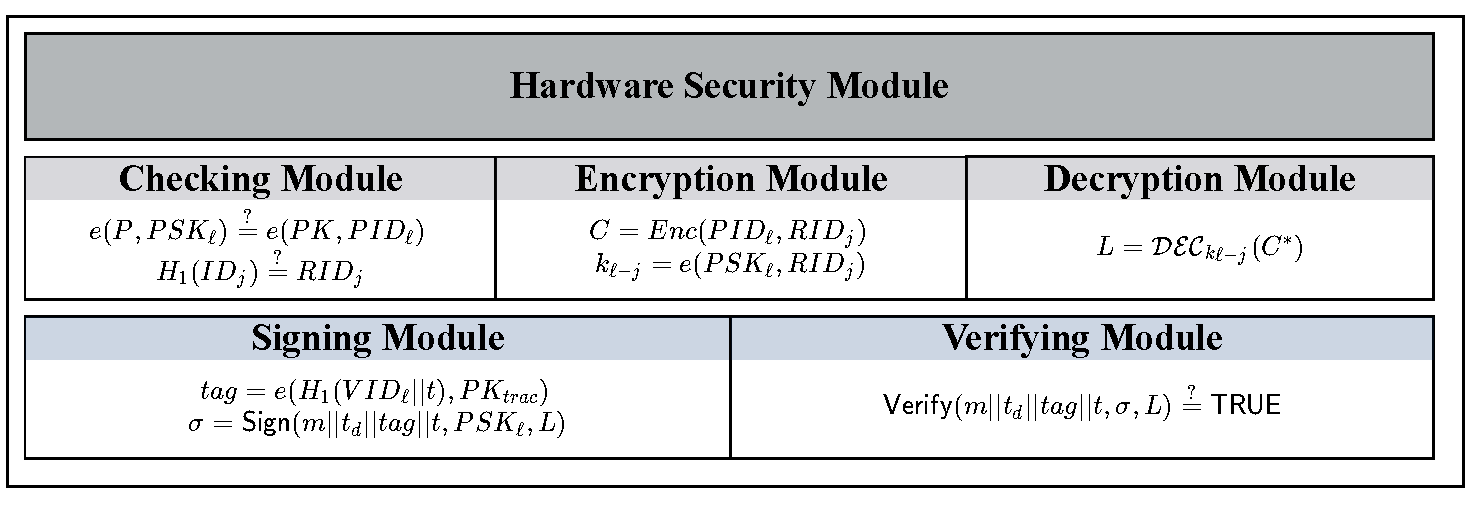
\includegraphics[width = 1.0\textwidth]{hsm}
\caption{组成HSM的各个模块}
\end{figure}

当TRC完成初始化工作之后,生成的公共参数$pp=(\mathbb{G}_1,\mathbb{G}_2,P,q,e,PK,H_1,H_2)$被预先载入到HSM模块中。从图中可以看出,当车辆$V_\ell$获取到自己的密钥对$(PID_\ell,PSK_\ell)$并将密钥对载入到HSM中时,HSM中的假名校验模块首先对这对密钥进行校验。

校验的过程就是检查以下等式是否成立:
\begin{equation}
e(P,PSK_\ell)\overset{?}{=}e(PK,PID_\ell)
\end{equation}
如果校验通过,那么HSM就可以载入这对密钥以进行后面的操作。

在成员列表分配阶段,车辆$V_\ell$在收到$RSU_j$的公钥$PID_j$之后,首先需要调用HSM的假名校验模块来校验$RSU_j$的公钥$PID_j$是否合法。
由于不同区域内的RSUs身份信息$ID_j$都是公开可查的,通过提供$PID_j$和$ID_j$给HSM,HSM只需要检查以下等式是否成立:
\begin{equation}
H_1(ID_j)\overset{?}{=}RID_j
\end{equation}
如果校验通过,HSM中的加密模块便自动使用$RID_j$作为加密的公钥对车辆的假名$PID_\ell$进行加密。即计算:
\begin{equation}
C=\mathsf{Enc}(PID_\ell,RID_j)=(rP,PID_\ell\oplus g_d^r)
\end{equation}
其中,$g_d^r=e(PID_\ell,PK)$。

在输入加密的密文之后,HSM还需要计算与$RSU_j$对应的共享密钥,即计算:
\begin{equation}
k_{\ell-j}=e(PSK_\ell,RID_j)
\end{equation}
并把此共享密钥作为解密模块的解密密钥。

在收到$RSU_j$返回的$(C^*,\Sigma,t_d)$之后,HSM的解密模块开始验证$t_d$是否失效,如果还未失效则再验证消息验证码$\Sigma$。在这些都通过验证之后,便可以使用对称解密算法$\mathcal{DEC}_{k_{\ell-j}}(C^*)$对密文$C^*$进行解密。
值得注意的是,在实际应用中,我们可以使用AES作为对称加解密算法,这类算法现在已经很成熟,计算效率比较高。

在完成了对成员列表的还原之后,签名模块便可以使用此列表$L$作为输入,并输出对消息$m$的一个环签名。
验证模块则是在收到其它车辆的签名信息后,利用验证算法$\mathsf{Verify}$完成对消息$m$的验证。

下面我们将对此方案满足的可验证性、匿名性、不可伪造性、可追踪性、抗重放攻击以及高效性分别进行说明。
为了方便描述,我们依然使用$V_\ell$代表进行签名的车辆,用$V_k$表示验证签名的车辆。

\subsection{可验证性}[authentication]

可验证性指的是,在此方案中如果所有过程都是正确执行的,那么最终得到的签名一定可以通过验证。
因此我们需要考虑成员列表分配过程以及签名和验证过程的正确性。
从前面的描述我们可以知道,$V_\ell$在向$RSU_j$请求成员列表时,发送给$RSU_j$的密文是:
\begin{equation}
C=(rP,V)=(rP,PID_\ell\oplus g_d^r)
\end{equation}
$RSU_j$在收到此密文后,计算$V\oplus e(RSK_j,rP)$,由于:
\begin{equation}
V\oplus e(RSK_j,rP)=V\oplus e(RID_j,s\cdot P)^r=V\oplus g_d^r=PID_\ell
\end{equation}
因此$RSU_j$能够正确获取车辆$V_\ell$的假名$PID_\ell$。
而$RSU_j$计算的共享秘钥为$k_{j-\ell}=e(PID_\ell,RSK_j)$,$VID_\ell$计算的共享秘钥为$k_{\ell-j}=e(PSK_\ell,RID_j)$,由双线性映射的性质可以得到:
\begin{equation}
e(PID_\ell,RSK_j)=e(PID_\ell,s\cdot RID_j)=e(s\cdot PID_\ell,RID_j)=e(PSK_\ell,RID_j)
\end{equation}
双方在这个交互过程中获取了相同的密钥,再根据对称密码体制的特点,从而保证$V_\ell$可以从$RSU_j$处正确获取成员列表信息。

对于车辆$V_\ell$以及成员列表$L=\{PID_1,PID_2,...,PID_n\}$ $(1\leq \ell\leq n)$,以及所需签名的信息$m$,我们可以令$m'=m||t_d||tag||t$。那么通过得到的签名$\sigma$为:
\begin{equation}
\sigma=(\cup_{i=1}^n\{U_i\},V)
\end{equation}
其中,对于$1\leq i\leq n$且$i\neq \ell$,$U_i$都是从$\mathbb{G}_1$中随机选取的,我们记$h_i=H_2(m'||L||U_i)$。计算完成后我们可以随机选取$r'_\ell \in_R\mathbb{Z}_q^*$,并计算$U_\ell=r'_\ell PID_\ell-\sum_{i\neq \ell}\{U_i+h_iPID_i\}$,$h_\ell=H_2(m'||L||U_\ell)$。最后可得到$V=(h_\ell+r'_\ell)PSK_\ell$。

在验证的过程中,对于$1\leq i \leq n$,车辆$V_k$首先计算$h_\ell=H_2(m'||L||U_i)$,那么根据双线性映射的性质,我们可以得到下面的等式:
\begin{equation}
\begin{split}
e(PK,\sum_{i=1}^n(U_i+h_iPID_i)) = & e(s\cdot P,U_\ell+h_\ell PID_\ell+\sum_{i=1,i\neq \ell}^n(U_i+h_iPID_i)) \\
 = & e(s\cdot P,r_\ell'PID_\ell+h_\ell PID_\ell)  \\
 = & e(s\cdot P,(r_\ell'+h_\ell)PID_\ell) \\
 = & e(P,(r_\ell'+h_\ell)PID_\ell\cdot s) \\
 = & e(P,V) \\
\end{split}
\end{equation}
因此,只要$V_\ell$正确执行相关的协议,那么产生的签名一定能够通过$V_k$的验证。

\subsection{匿名性}[anonymous]

我们主要从V2I和V2V两个角度分析匿名性,从V2I的角度,由于$RSU_j$是半诚实的,在与车辆$V_\ell$的通信过程中,它唯一知道的就是车辆$V_\ell$的公钥,即$PID_\ell$。
由于$PID_\ell$是由TRC生成的,且$PID_\ell=H_1(VID_\ell||salt)$。
根据密码哈希函数的单向性,在只知道$PID_\ell$的情况下,$RSU_j$能在概率概率多项式时间内找到一个$ID$使得$H_1(ID)=PID_\ell$的概率是可以忽略不计的。
而且我们建议车辆的公钥需要定时更新,由此保证了$RSU_j$无法将$PID_\ell$与车辆的真实身份关联起来。

从V2V的角度,由于我们选择的是由Chow,Yiu和Hui提出的基于身份的环签名方案,这种环签名方案具有完全的匿名性,因此在知道车辆$V_\ell$生成的签名$\sigma$的情况下,车辆$V_k$根据列表$L$只能推断出签名者在列表$L$内这条信息,并不能推断出签名者具体是列表中的哪一位。这样就能够很好地保证签名者的匿名性。
另外,在广播的信息中还存在可追踪的标签,即$tag=e(H_1(VID_\ell||t),PK_{trac})$。
密码哈希函数的性质保证了车辆$V_k$不能根据$tag$的值从中获取到有用的信息。

\subsection{不可伪造性}[non-repudiation]

在前面的假设中,我们假定RSUs是不完全受信任的,也就是说RSUs不会篡改或伪造数据,因此我们在考虑不可伪造性时,只需要考虑系统中的恶意车辆。
与前面分析类似,我们分别从V2I与V2V两个方面进行说明。

在V2I的过程中,假设有一恶意的车辆$VID_{i'}$想伪装成$VID_\ell$并与$RSU_j$进行通信。
假设$VID_{i'}$已经知道了$VID_\ell$的公钥为$PID_\ell$,那么$RSU_j$向他返回的就是用$k_{j-\ell}$加密的信息。
由于我们使用的是对称密码体制,并且采用Encrypt-then-MAC的模式。
这种模式是满足选择密文安全的,也就是说$V_{i'}$在没有密钥$k_{j-\ell}$的情况下不能获取到任何有用的信息。
因此我们只需要证明$V_{i'}$在只知道$PID_\ell$的情况下对它获取到密钥$k_{j-\ell}$没有任何帮助。
下面我们使用基于游戏(Game-Based)的方式进行证明。

假设挑战者$\mathcal{C}_1$与攻击者$V_{i'}$进行下面这个游戏$Game_1$:
\begin{itemize}
  \item[1.] 挑战者$\mathcal{C}_1$生成参数$pp=(\mathbb{G}_1,\mathbb{G}_T,P,q,e,PK,H_1)$和主密钥$s$,并随机挑选两个ID:$ID_1\in_R\mathbb{Z}_q^*$,$ID_2\in_R\mathbb{Z}_q^*$,令$PID_\ell:=H_1(ID_1),RID_j:=H_1(ID_2)$。最后将$(pp,PID_\ell,RID_j)$发送给攻击者$V_{i'}$;
  \item[2.] 挑战者$\mathcal{C}_1$选择一个比特$b\in_R\{0,1\}$,如果$b=0$,则令$h:=k_{j-\ell}$;如果$b=1$,则随机选取$h\in_R\mathbb{G}_T$。挑战者将$h$发送给攻击者$V_{i'}$;
  \item[3.] 攻击者收到$h$之后,在多项式时间内返回一个比特$b'$;
  \item[4.] 挑战者$\mathcal{C}_1$判断$b'$是否等于$b$,若$b'=b$,则称攻击者$V_{i'}$成功;如果$b'\neq b$,则称其攻击失败。
\end{itemize}

在进行多项式次数后,我们用$\Pr[\mathsf{Game}_1(V_{i'})=1]$表示攻击者$V_{i'}$在$Game_1$中获胜的概率。

类似地,我们假设有挑战者$\mathcal{C}_2$与攻击者$\mathcal{A}$进行下面的游戏$Game_2$:
\begin{itemize}
  \item[1.] 挑战者$\mathcal{C}_2$生成参数$pp=(\mathbb{G}_1,\mathbb{G}_T,P,q,e,PK,H_1)$和主私钥$s$,并随机选取$a\in_R\mathbb{Z}_q^*,b\in_R\mathbb{Z}_q^*$,令$y_1=a\cdot P,y_2=b\cdot P$。最后将$(pp,y_1,y_2)$发送给攻击者$\mathcal{A}$;
  \item[2.] 挑战者$\mathcal{C}_2$选择一个比特$b\in_R\{0,1\}$,如果$b=0$,则令$h:=e(y_1,y_2)^s$;如果$b=1$,则随机选取$h\in_R\mathbb{G}_T$。$\mathcal{C}_2$将$h$发送给攻击者$\mathcal{A}$;
  \item[3.] 攻击者$\mathcal{A}$接收到$h$后,在多项式时间内返回一个比特$b'$;
  \item[4.] 挑战者$\mathcal{C}_2$判断$b'$是否与$b$相等,若$b'=b$,则称攻击者$\mathcal{A}$攻击成功;否则称$\mathcal{A}$攻击失败。
\end{itemize}

在进行多项式次数后,我们用$\Pr[\mathsf{Game}_2(\mathcal{A})=1]$表示攻击者$\mathcal{A}$在$Game_2$中获胜的概率。

由DBDH问题的定义,我们把在$Game_2$中获胜看做解决一个DBDH问题。
由于我们假设DBDH问题是一个困难问题,那么存在一个可忽略函数$\mathsf{negl}(\kappa)$,使得:
\begin{equation}
|\Pr[\mathsf{Game}_2(\mathcal{A})=1]-\frac{1}{2}|\leq\mathsf{negl}_1(\kappa)
\end{equation}
始终成立。

由于$H_1$是一个Map-to-Point的密码哈希函数,在随机预言机模型的假设下,我们可以得到:
\begin{equation}
|\Pr[\mathsf{Game}_1(V_{i'})=1]-\Pr[\mathsf{Game}_2(\mathcal{A})=1]|\leq \mathsf{negl}_2(\kappa)
\end{equation}
由公式(4-12)与(4-13),我们可以推出:
\begin{equation}
|\Pr[\mathsf{Game}_1(V_{i'})=1]-\frac{1}{2}|\leq \mathsf{negl}_1(\kappa) + \mathsf{negl}_2(\kappa)
\end{equation}

也就是说,$V_{i'}$在$Game_1$中能取得成功的概率与随机选取一个比特的概率是基本相同的。即在随机预言机模型的假设下,$V_{i'}$在只知道$PID_\ell$与$RID_j$的情况下无法获取到共享秘钥$k_{j-\ell}$的任何信息。

在V2V的过程中,签名$\sigma$是由HSM计算并输出的,签名的内容是$m||t_d||tag||t$。
由于我们使用的签名方案具有适应性选择消息和身份下的存在性不可伪造的特性,因此恶意的车辆$V_{i'}$对$(t_d,tag,t,L)$中任一内容进行伪造都将通过不了验证。

\subsection{可追踪性}[traceability]

在一些特殊情况下,如出现意外事故的情况下,执法机关将有必要调查事故中信息的真正签名者。
假设车辆$V_{i'}$发送的消息为$m$,对应的签名为$\sigma$。
我们知道,车辆$V_{i'}$发送的信息中还包括一个可追踪的$tag$,且
\begin{equation}
tag=e(H_1(VID_{i'}||t),PK_{trac})
\end{equation}
执法机关首先将$(L,t)$提交给TRC,其中$L=\{PID_1,PID_2,...,PID_n\}(1\leq i'\leq n)$。
之后计算$tag'$,即:
\begin{equation}
tag'=tag^{1/s_{trac}}=e(H_1(VID_{i'}||t),s_{trac}^{-1}PK_{trac})=e(H_1(VID_{i'}||t),P)
\end{equation}
而TRC返回的为一个列表,即:
\begin{equation}
L'=\{e(H_1(VID_1||t),P),e(H_1(VID_2||t),P),...,e(H_1(VID_n||t),P)\}
\end{equation}
由于$1\leq i'\leq n$,因此$tag'$一定属于列表$L'$,那么也就是说一定可以根据$tag'$和$L'$来判断出签名者的假名$PID_{i'}$。
在找到$PID_{i'}$之后,执法机关也可以进一步通过向TRC发出请求还原出$PID_{i'}$对应的真实身份$VID_{i'}$,并完成撤销等一系列操作。
因为$tag$的不可伪造性(根据前面的论述以及HSM的特性),通过这个过程一定可以找到真正的签名者,而且所需要的时间与$L$的长度成正比。

对于TRC来说,它在不知道$tag$的情况下,仅仅根据执法机关递交的$(L,t)$的信息无法判断出执法机关所需要还原的签名者的身份。
执法机关只有在真正确定该车辆为恶意车辆的情况下,才会向TRC请求还原其真实的身份,从某种意义上来说也是避免了在未真正确定事故真相之前过早暴露车辆身份。

\subsection{抗重放攻击}[reply-attack colli]

重放攻击(Replay Attack)指的是恶意用户通过收集合法有效的数据信息并加以重复使用以达到伪装成真实用户的目的。
一般我们使用添加时间戳的方法阻止网络环境中的重放攻击。
由于车辆自组网处在一个公开的网络环境中,车辆之间发送的信息大多以广播的形式传送,因此很容易被其它恶意的用户或车辆进行收集。不附加时间戳的话,车辆发送的信息很方便被其它网络节点利用。

在我们的方案中,假设恶意车辆$V_{i'}$在收到了广播信息$(m,\sigma,L,t_d,t,tag)$之后,尝试再隔一段时间重复广播此信息。
由于广播信息中包含了签名时生成的时间戳$t$,如果$V_{i'}$不做任何修改直接发送信息$(m,\sigma,L,t_d,t,tag)$的话,则会因为当前时间与$t$相差太大而通不过其它车辆的校验;
如果$V_{i'}$尝试修改$t$为当前时间,又因为$\sigma=\mathsf{Sign}(m||t_d||t||tag||t,PSK_\ell,L)$,也会通不过其它车辆的验证。
因此,在这种对实时性要求比较高的车辆自组网环境中,$t$的存在一方面可以确保消息$m$的时效性,另一方面可以防御重放攻击。
要能有效地抵抗重放攻击,一个比较重要的条件是车辆自组网中的设备需要准确的时间同步。

\subsection{高效性}[efficient]

由于我们的方案是在双线性映射上进行的,首先我们需要对双线性映射上相关操作的运算时间进行估算。
下面的测试是在搭载英特尔酷睿i7-6700处理器的Linux 64位系统环境中进行的,调用的是基于Python语言的CHARM库\cite{charm13}。
特别地,我们使用的是512位椭圆曲线,对其上面的每个操作分别进行了10000次随机运算,并将运行消耗的CPU时间取平均值。
最终我们把比较耗时的运算列举出来,如表4-4所示。

\begin{table}[htbp]
\bicaption[table3]{}{双线性映射上单个操作的运算耗时}
\vspace{0.5em}\centering\wuhao
\begin{tabular}{ccccc}
\toprule[1.5pt]
 符号 & 描述 & CPU时间(单位:ms)\\
\midrule[1pt]
 $T_{bp}$ & 执行一次双线性映射计算的时间 & 0.718 \\
 $T_{ep}$ & 对$\mathbb{G}_T$中的元素执行一次指数运算所需的时间 & 1.228 \\
 $T_{em}$ & 对$\mathbb{G}_1$上的点执行一次标量乘法所需的时间 & 1.245 \\
 $T_{mph}$& 执行一次Map-to-Point哈希函数所需的时间 & 2.606 \\
\bottomrule[1.5pt]
\end{tabular}
\end{table}

其他的操作,如椭圆曲线上的加法,哈希函数$H_2$,对称加密解密算法及MAC运算所需时间较短,相较上表中的可以忽略不计。
我们用$n$来表示环签名中列表成员的数量,当$n=10$的情况下,各个阶段所需要花费的时间如表4-5所示。

\begin{table}[htbp]
\bicaption[table4]{}{方案中各个阶段所需时间(单位:ms)}
\vspace{0.5em}\centering\wuhao
\begin{tabular}{cccc}
\toprule[1.5pt]
 & TRC & RSU & OBU \\
\midrule[1pt]
初始化:& $T_{em}\approx 1.245$ & - & - \\
密钥生成:& $T_{mph}+T_{em}\approx 3.851$ & - & - \\
列表分发:& - & $T_{bp}\approx 0.718$ & $2T_{bp}+T_{ep}\approx 2.664$ \\
签名: & - & - & $(n+1)T_{em}+T_{bp}\approx 14.940$ \\
验证: & - & - & $2T_{bp}+nT_{em}\approx 15.131$\\
\bottomrule[1.5pt]
\end{tabular}
\end{table}

从表中我们可以看到,主要是签名和验证的过程花费的时间比较长,且消耗的时间与使用的列表长度成正比。
因此,需要进一步对比近些年其他基于环签名的方案中\cite{chaurasia2011conditional,zeng2015privacy}签名和验证所需要的时间。如表4-6所示,我们列举了在签名以及验证两个方面与其他基于环签名的方案的对比。

\begin{table}[htbp]
\bicaption[table5]{}{与其他基于环签名的方案的对比(单位:ms)}
\vspace{0.5em}\centering\wuhao
\begin{tabular}{ccc}
\toprule[1.5pt]
 & 签名所需时间 & 验证所需时间 \\
\midrule[1pt]
方案IV\cite{chaurasia2011conditional} & $2T_{bp}+2T_{ep}+(2n+2)T_{em}\approx 31.282$ & $T_{bp}+2(n+1)T_{ep}\approx 26.506$ \\
方案V\cite{zeng2015privacy} & $3T_{bp}+4T_{ep}+2nT_{em}+2T_{mph}\approx 37.178$ & $3T_{bp}+3T_{ep}+(n+2)T_{em}\approx 20.778$\\
我们的方案 & $(n+1)T_{em}+T_{bp}\approx 14.940 $ & $2T_{bp}+nT_{em}\approx 15.131$ \\
\bottomrule[1.5pt]
\end{tabular}
\end{table}

通过对比我们发现,该方案在签名方面所需的时间要明显低于另外两个方案。
正如前面介绍的,在IEEE80.2.11p标准中,DSRC技术要求车辆以100到300毫秒的时间间隔广播与交通有关的信息。
而在我们方案中,当环签名中成员为10个的时候,签名与验证消耗的时间为15毫秒左右,为了应对车辆比较密集的场景,我们建议由RSUs自动调整签名的成员个数。
比如当车辆比较多的时候,RSUs可以减少环中的成员个数,以保证系统的高效运行;当车辆比较少的时候,RSUs可以适当增加环中成员的个数,以便更好地保护车辆的隐私。

\section{本章小结}[Summary IV]

这一章我们首先介绍了车辆自组网的概念,简单概括了车辆自组网的各个角色及它们之间的通信方式。
然后通过介绍主流的通信标准,我们发现当前这些标准主要关注的是信息的可验证性,缺少对车辆隐私的保护措施。
因此最近提出的方案都是围绕着系统的安全性,车辆的匿名性、网络的实时性和对消息的可追踪性这几个基本特性。
在给出提出的方案之前,我们先对这些相关的解决方案进行了整理分类,并说明了这些方案的局限性。
再结合与基于属性的凭证系统的对比,我们决定使用具有匿名性质的签名来构造这样一个功能完备的方案。
对于V2V,我们使用环签名的方式来保证通信过程中消息的可验证性及车辆身份的匿名性。
相较于其他基于环签名的方案,我们的方案充分发挥了RSUs的作用,并利用RSUs保证了签名的可靠性。
为了将RSUs合理地融入到车辆自组网的环境中,我们结合了基于身份的密码学以及对称密码体制的优势,在保证效率的同时满足了车辆自组网中对效率的需求。
为了更好地进行说明,我们将车辆网中参与交互的实体分为了TRC、执法机关、配备了OBUs的车辆和固定区域内的RSUs这四类。
它们分别执行不同的功能。
TRC负责系统参数的生成和假名的生成,RSUs负责向该区域内的车辆分配成员列表,车辆在获取到列表后便可以使用环签名的方式完成信息的签名与认证。
执法机关与TRC合作可以还原出签名者的真实身份。

我们的方案与其它方案相比最大的优势是车辆不用频繁地更换自己的假名,因此OBUs设备就不用提前存储太多的假名,也不需要担心因为更换假名带来的隐私泄漏问题。
另外我们的方案对RSUs设备的依赖也比较弱,避免了因为RSUs有限的性能带来的网络传输瓶颈问题。
在追踪的过程中引入了执法机关,并且使用执法机关与TRC合作的方式来还原签名者的真实身份。
这样的做法比较符合实际中的场景,同时也在最大程度上保护了用户的隐私。

在这一章的最后,我们将提出的方案与其他基于环签名的方案进行了对比,结果显示在成员个数相同的情况下,我们的方案所需要的计算时间更短。
而且在我们的方案中,RSUs可以根据当前的网络情况对成员个数进行动态的调整,进而确保在不同情境中既能保护用户的隐私,也能确保签名和验证的效率。
综合这些特性,我们提出的方案能适用于像车辆自组网这种对实时性要求比较高的场景。